\subsection{Minimum Vertex Cover}
The network consists of two graph convolutional layers, each consisting of an MLP with 1 layer of 100 hidden nodes.
This the output is activated through the sigmoid function, through a final graph convolution.

Firstly, the model is trained on a singular graph.
This graph is randomly generated through the \verb|networkx| package, consisting of 100 nodes.
Each edge has a $5\%$ probability of being included in the graph.
After 653 epochs, the model converges, taking approximately 1 second.
Note that the models are run in a Jupyter Notebook on an M1 mac, and the runtimes are therefore not directly comparable with other methods.

The vertex cover is shown in \autoref{fig:mvc_single_graph_random}, having a size of $61$ coloured nodes, satisfying all constraints.
Additionally the number of unnecessary nodes are computed, being the number of colored nodes only connected to other colored nodes.

\begin{figure}[h]
    \centering
    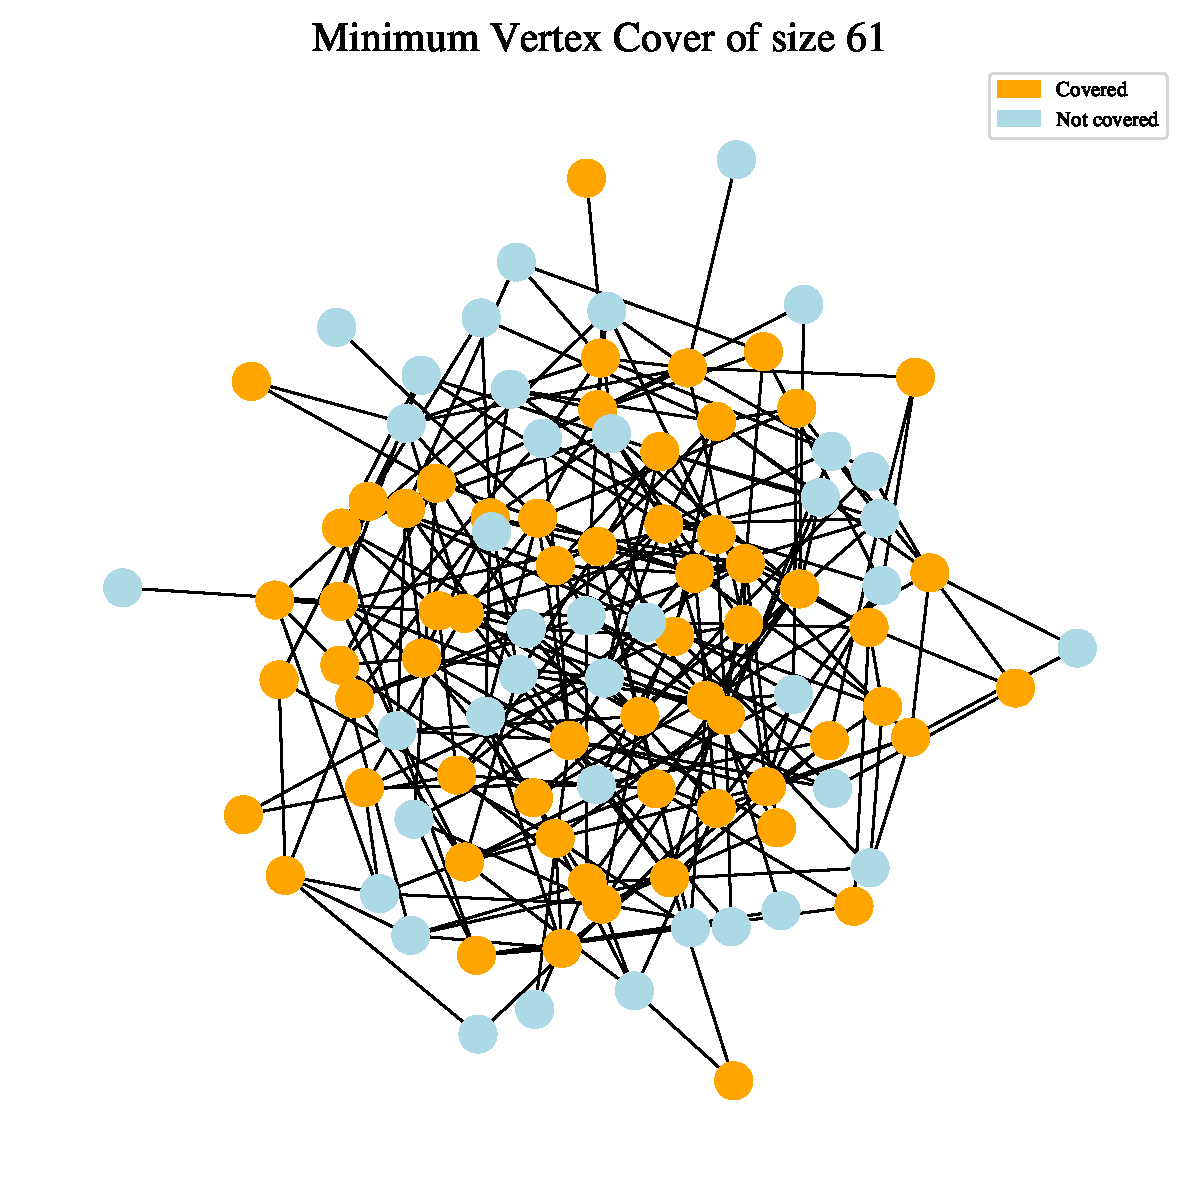
\includegraphics[width=\linewidth]{Project2TSP/_src/figures/mvc_graph_single.pdf}
    \caption{Model trained on a single random graph. Orange nodes are covered, blue are not.}
    \label{fig:mvc_single_graph_random}
\end{figure}

On such a small sample, the model is likely to be sensitive to the initial conditions of the model.
Therefore, the model is initialised on 100 random seeds, each trained on the same initial graph.
The results are presented in \autoref{table:mvc_single_seed}, showing that the model is consistently predicting a cover of around $61$.

\begin{table}[h!]
\centering
\caption{Model sensitivity to initial seed.}
\begin{tabular}{c|c|c|c}
    \toprule
    \# of & & edge & unnecessary \\
    occurrences & size & violations & colorings \\
    \colrule
    69 & 61 & 0 & 0 \\
    19 & 60 & 0 & 0 \\
    9 & 62 & 0 & 0 \\
    1 & 59 & 0 & 0 \\
    1 & 62 & 0 & 1 \\
    1 & 99 & 0 & 39 \\
    \botrule
\end{tabular}
\label{table:mvc_single_seed}
\end{table}

The predicted cover sizes are compared against the local-ratio algorithm \cite{local_ratio_approx}, guaranteeing an approximate solution which is at most twice as large as the optimal covering.
For this initial graph, the approximate cover consists of $80$ nodes, meaning our model is able to outperform it.

Finally, the model is trained on two sets of $100$ graphs, with the first being random with probability $5\%$, and the second being $3$-regular.
The models then predicts a cover for two sets of unseen graphs, being another set of random and regular graphs.
In \autoref{fig:mvc_train_random} we see that the model is able to consistently predict valid solutions, beating the approximate solution in all cases.
However, it is not able to generalise well for unseen graphs.

\begin{figure}[h]
    \centering
    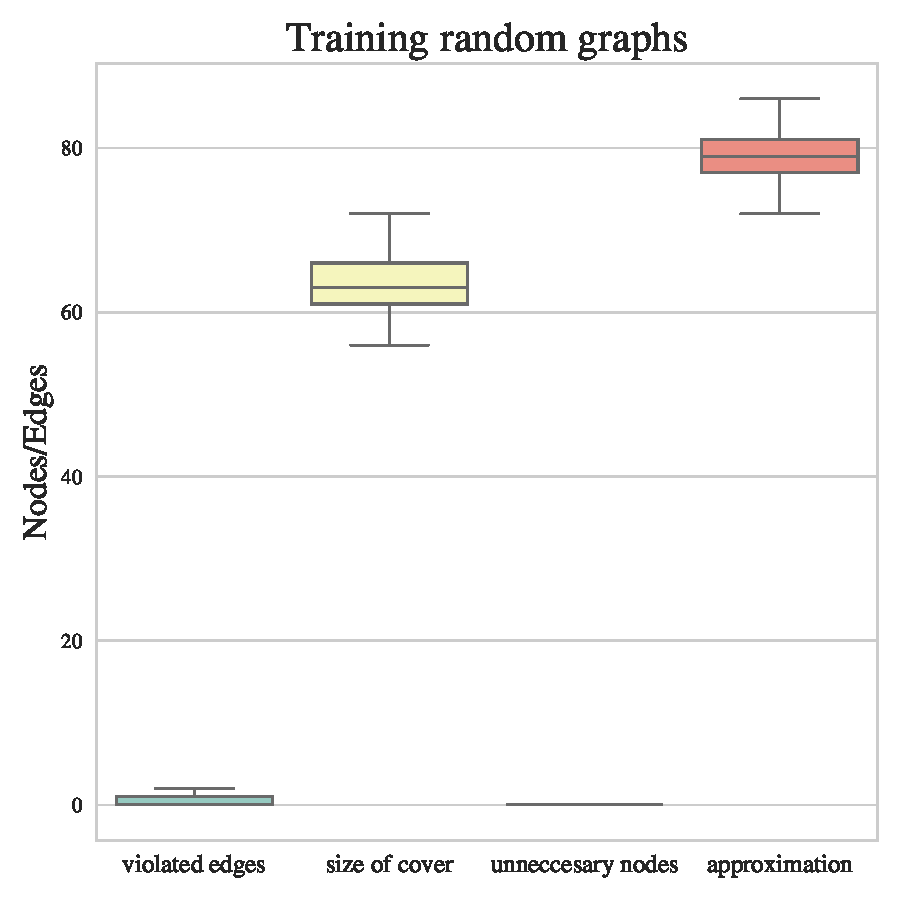
\includegraphics[width=\linewidth]{Project2TSP/_src/figures/mvc_train_random.pdf}
    \caption{MVC results from training on 100 random graphs.}
    \label{fig:mvc_train_random}
\end{figure}

In \autoref{fig:mvc_random_to_random} and \autoref{fig:mvc_random_to_regular}, this model is evaluated against respectively random and regular graphs.
The model is rarely able to predict valid solutions, and those which are valid are worse than the approximations.
Notably, the model seems to perform better on the $3$-regular graphs than on the random ones.

\begin{figure}[h]
    \centering
    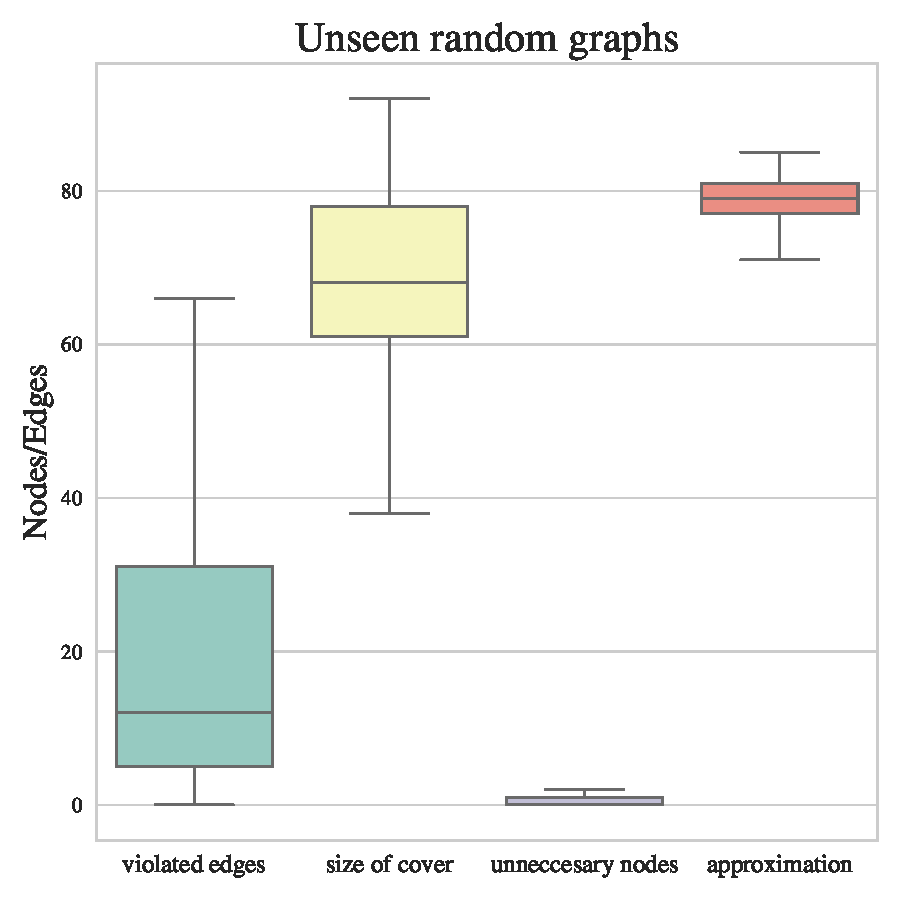
\includegraphics[width=\linewidth]{Project2TSP/_src/figures/mvc_random_to_random.pdf}
    \caption{MVC predictions on 100 random graphs, from training on 100 random graphs.}
    \label{fig:mvc_random_to_random}
\end{figure}

\begin{figure}[h]
    \centering
    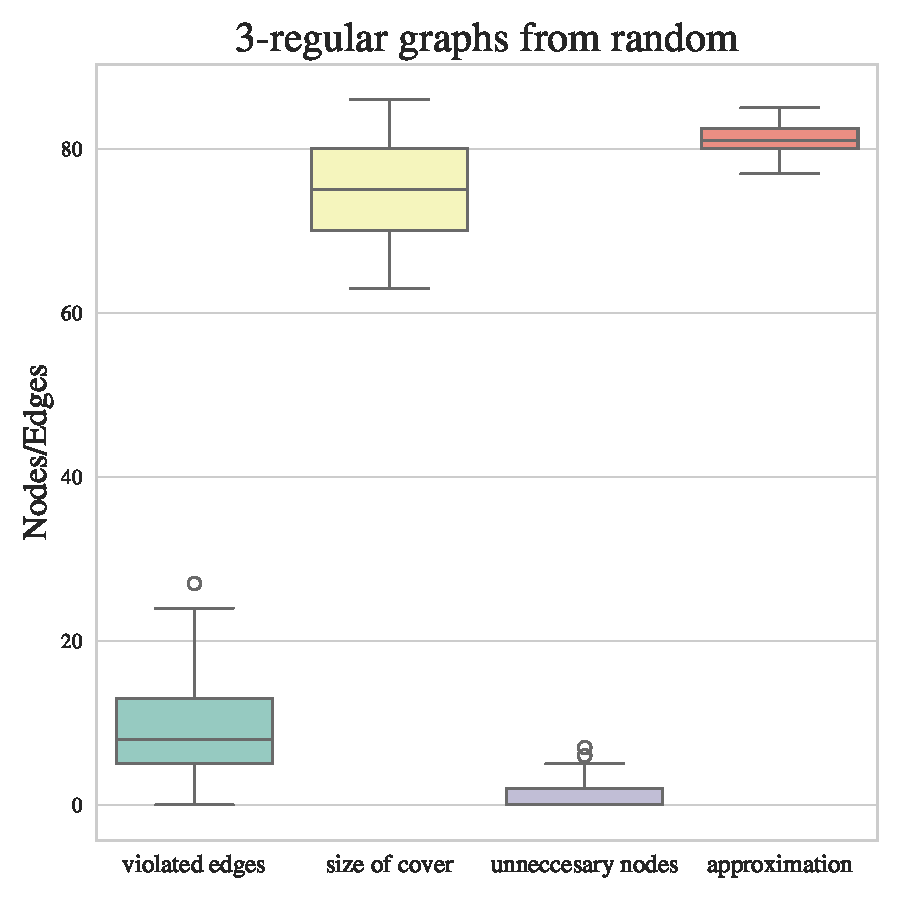
\includegraphics[width=\linewidth]{Project2TSP/_src/figures/mvc_random_to_regular.pdf}
    \caption{MVC predictions on 100 $3$-regular graphs, from training on 100 random graphs.}
    \label{fig:mvc_random_to_regular}
\end{figure}

\begin{figure}[h]
    \centering
    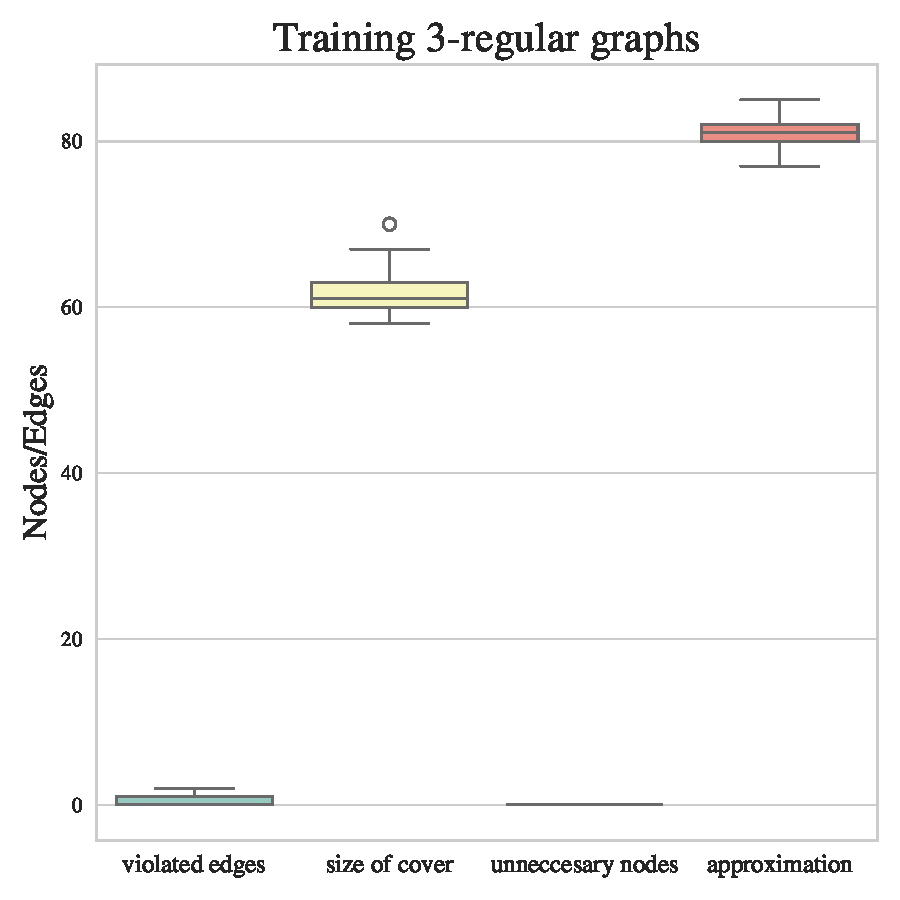
\includegraphics[width=\linewidth]{Project2TSP/_src/figures/mvc_train_regular.pdf}
    \caption{MVC results from training on 100 $3$-regular graphs.}
    \label{fig:mvc_train_regular}
\end{figure}

Training the model on $3$-regular graphs instead, as in \autoref{fig:mvc_train_regular}, the model is again able to outperform the approximations.
It seems to perform slightly worse unseen $3$-regular graphs in \autoref{fig:mvc_regular_to_regular}, and a lot worse on the unseen random graphs in \autoref{fig:mvc_regular_to_random}.


\begin{figure}[h]
    \centering
    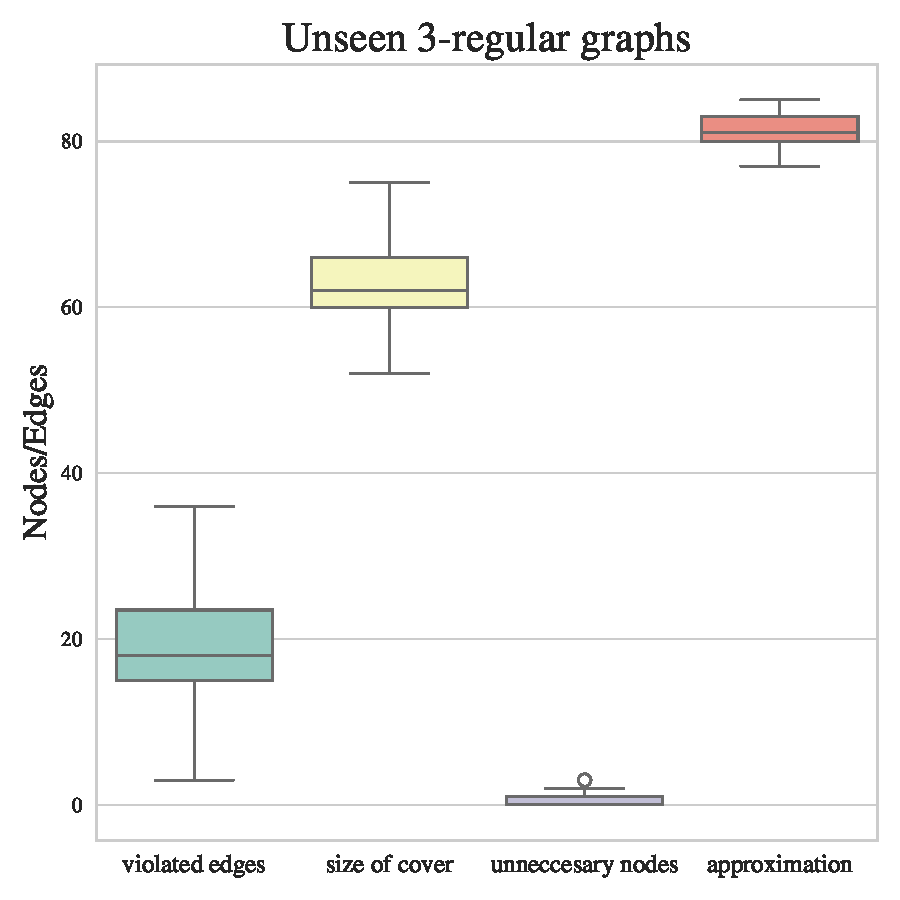
\includegraphics[width=\linewidth]{Project2TSP/_src/figures/mvc_regular_to_regular.pdf}
    \caption{MVC predictions on 100 $3$-regular graphs, from training on 100 $3$-regular graphs.}
    \label{fig:mvc_regular_to_regular}
\end{figure}

\begin{figure}[h]
    \centering
    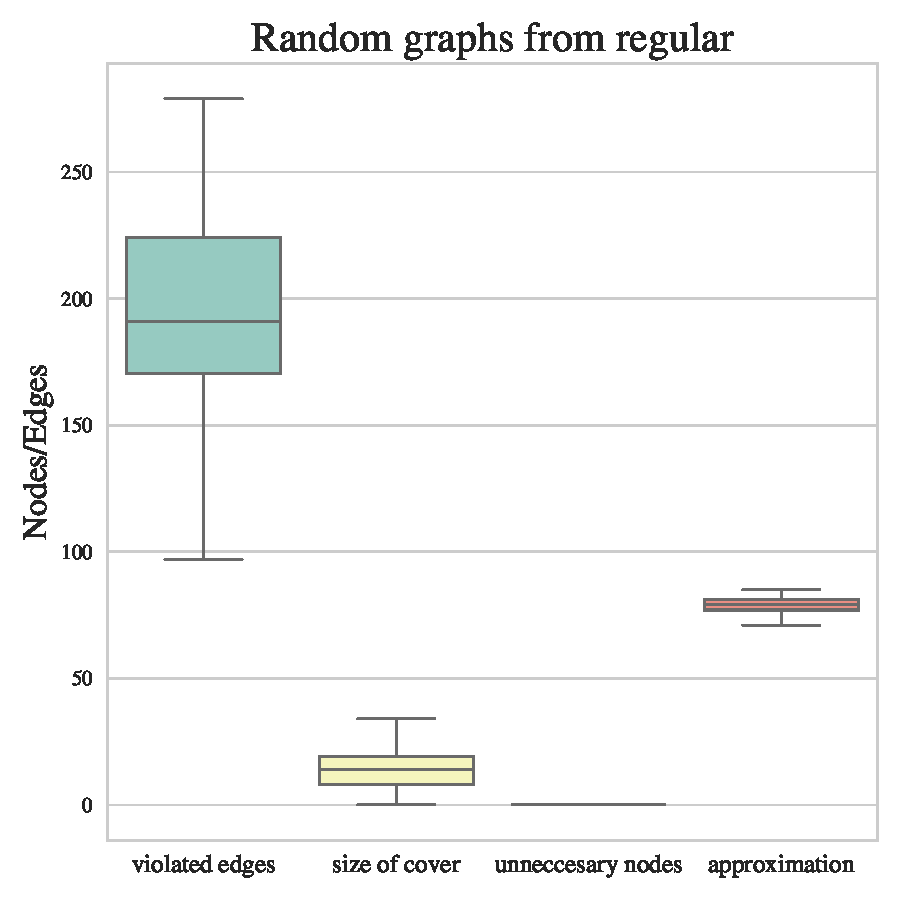
\includegraphics[width=\linewidth]{Project2TSP/_src/figures/mvc_regular_to_random.pdf}
    \caption{MVC predictions on 100 random graphs, from training on 100 $3$-regular graphs.}
    \label{fig:mvc_regular_to_random}
\end{figure}

Due to memory constraints, the size of the training set was rather limited, perhaps explaining the poor generalisation.
However, given the fact that the generated solutions are purely attained through training the models without prior knowledge, the results from the training sets are perhaps a valid measure of the models performance.

\subsection{Hamiltonian cycles}
Although the objectives of finding a Hamiltonian cycle in a graph and determining the route of a traveling salesman seem similar, the problems are in practice much less related.
When looking for a Hamiltonian cycle, one typically starts with a sparser graph.
An example of this could be a social graph of who knows who, where the aim is to pass a message around to each person.

On the other hand, TSP typically concerns itself with complete graphs, or nearly so.
As discussed previously, GCNs are not able to function on complete graphs due to oversmoothing.
Finding a Hamiltonian cycle in a complete graph is a trivial exercise, simply take an arbitrary ordering of the nodes.

Due to this, the immediate choice of training data was rather limited.
Because of this, $2N \times 2N$ grids of points was chosen, as it is guaranteed to have Hamiltonian cycles while being relatively sparse \cite{OEIS_hamilton}.

The models were trained on grids where nodes are connected to their orthogonal neighbours, as well as grids which were connected to their diagonal neighbours as well.
As the orthogonal grids are the ones described previously, and as they contain Hamiltonian cycles while being subgraphs of the diagonal ones, the diagonal graphs are also guaranteed to contain a Hamiltonian cycle.

The models were trained both with and without the TSP term of \eqref{eq:Hamilton_TSP}, in order to see if it had a meaningful effect.
The models struggled to converged, and therefore consisted of 1 convolution with an MLP of 32 nodes, before using the softmax function in the final prediction layer.
After this, the predictions were post processed such that $x_{1,1} = 1$, while $x_{i, 1} = x_{1, i} = 0$ for $i = 2, 3, \ldots, n$, in effect fixing that the first node should be the first in the cycle.
This should not have a cycle, as it does not matter which node is first.

As we see in \autoref{fig:8x8_chess_tsp} and \autoref{fig:8x8_chess_ham}, the addition of the TSP term does not seem to have had a meaningful effect.
This was a recurring theme across multiple different graphs, as well as with different model architectures.

\begin{figure}[h]
    \centering
    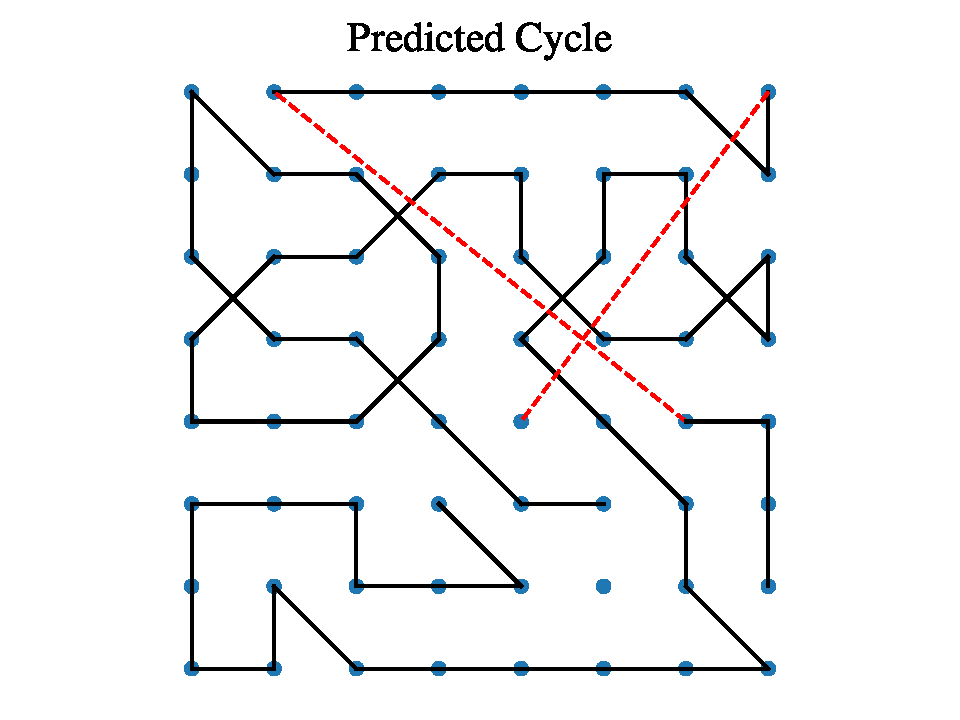
\includegraphics[width=\linewidth]{Project2TSP/_src/figures/tsp_8_chess_tsp.pdf}
    \caption{Model trained on $8 \times 8$ diagonal graph, with TSP.}
    \label{fig:8x8_chess_tsp}
\end{figure}

\begin{figure}[h]
    \centering
    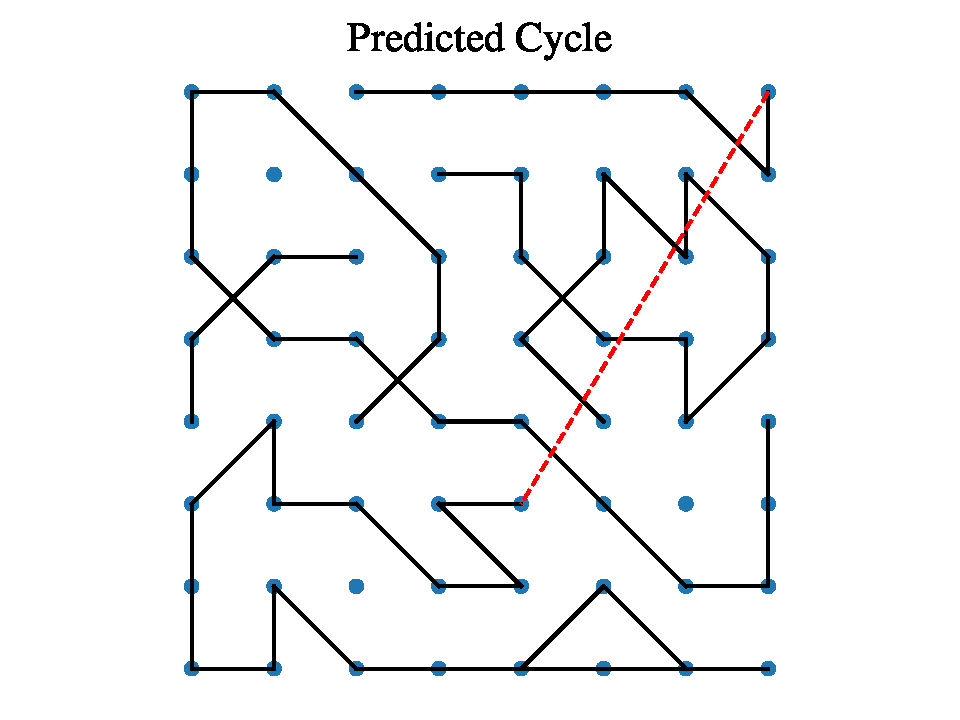
\includegraphics[width=\linewidth]{Project2TSP/_src/figures/tsp_8_chess_ham.pdf}
    \caption{Model trained on $8 \times 8$ diagonal graph, without TSP.}
    \label{fig:8x8_chess_ham}
\end{figure}

As we see, the model was not able to predict a valid tour in any case.
This is likely to stem from the approach used, as it is attempting to globally predict a route, consisting of $n^2$ variables.
It seems to be improving different line segments at once, running into an issue when they cannot be extended further.
This might be due to the fact that the line segments need to be constructed in order, beginning at an index $j$ in the cycle.
While the start and end of two lines might lie adjacent visually, if the corresponding indices do not match up, they cannot be connected with this method.
In this way, the model falls into a deep local minima.
Without major changes to the fundamental framework, I fail to see how this challenge can be overcome.

\textcite{joshi2019efficient} used a method not too unlike the one described here.
Their method predicts probabilities $x_{u,v}$, denoting the probability that nodes $u$ and $v$ should be connected.
They overcame the problem of oversmoothing through utilizing the $k$-nearest neighbour subgraph, training their network on a labeled data set.
As they do not the predicted ordering of the nodes, they decoded the probabilities using beam search in order to obtain a valid cycle.
The use of a labeled set limited their training to graphs with maximally 100 nodes, generalizing poorly with respect to larger graphs.
As they note in their paper, the use of heavy post processing might obscure the flaws of the model, which might be akin to what is seen in the models here.

\textcite{FELLEK2024127392} utilized deep reinforcement learning in combination with an adapted Graph Attention Network (GAT) in their proposed Gated Deep Graph Attention Network (G-DGANet).
In this method, the final tour is also constructed iteratively.
Their model generalized better for larger graphs, as well as outperforming a number of other machine learning methods.

